%% -*- Mode: LATEX -*-

\documentclass[12pt]{../rhitcsse}
\usepackage{multicol}
\usepackage{graphicx}

\ifx\CSSETHREEFIFTYTWO\undefined
\newcommand*{\CSSETHREEFIFTYTWO}{}
\course{CSSE 352}
\coursename{Video Game Development}
\term{Spring}
\acyear{2024-2025}
\instructor{Robert Williamson}
\fi

% Local Variables:
% mode:latex
% End:

 
\title{Lesson 8 Worksheet}

\makeatletter
\renewcommand{\labelenumi}{\bf Question \@arabic\c@enumi}
\makeatother

\begin{document}

\maketitle

\vspace*{0.15in}\hspace{0.25in}Name:\hrulefill\hspace{0.25in}\hspace{0.25in}

\begin{enumerate}
  \item What is the Singleton pattern used for?
  \vfill
  \item Our GameManager object is in the root of the hierarchy in the editor. 
  When the game starts, however, it moves. What is its parent?
  \vfill
  \item What kinds of bugs can overuse of Singletons lead to?
  \vfill
  \clearpage
  \centering
  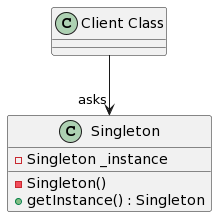
\includegraphics[width=0.25\textwidth]{../figs/Singleton.png}

\end{enumerate}

\end{document}

% Local Variables:
% mode:latex
% End:
